\documentclass[border=6pt]{standalone}
\usepackage[fontset=fandol]{ctex}
\usepackage{amsmath,amssymb,tikz}
\usetikzlibrary{arrows.meta,calc,decorations.pathmorphing}
\begin{document}

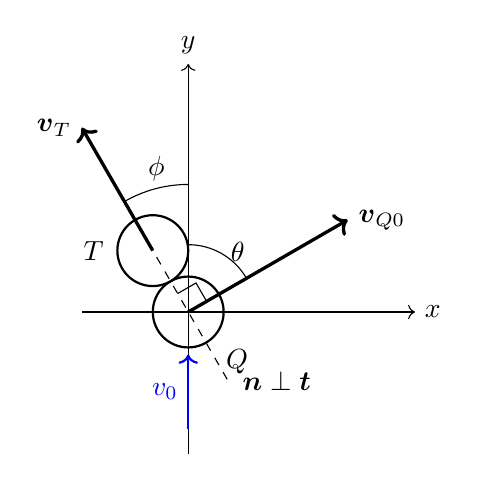
\begin{tikzpicture}[scale=.9]
\draw[->](-1.5,0)--(3.2,0)node[right]{$x$};
\draw[->](0,-2)--(0,3.5)node[above]{$y$};
\draw[thick](0,0)circle(.5)node[below right=10pt]{$Q$};
\draw[thick](-.5,.866)circle(.5)node[left=14pt]{$T$};
\draw[dashed](-1.5,2.6)--(.55,-.95);
\draw[->,very thick](-.5,.866)--(-1.5,2.598)node[left]{$\boldsymbol v_T$};
\draw[->,very thick](0,0)--(2.25,1.30)node[right]{$\boldsymbol v_{Q0}$};
\draw[->,blue,thick](0,-1.65)--(0,-.6)node[left,midway]{$v_0$};
\draw(0,1.8)arc(90:120:1.8);\node at(-.45,2.02){$\phi$};
\draw(0,.95)arc(90:30:.95);\node at(.7,.85){$\theta$};
\draw(-.15,.2598)--(.1098,.4098)--(.2598,.15);
\node[below]at(1.25,-.7){$\boldsymbol n\perp\boldsymbol t$};
\end{tikzpicture}

\end{document}
